
\documentclass{beamer}

\mode<presentation>
{ \usetheme{Antibes} }

\usepackage{times}
\usepackage{graphicx}

\title{Better hacking with Vim}
\author{Adrien Thebo \\
    Department of Computer Science \\
    Portland State University
}

\AtBeginSection[]
{
\begin{frame}<beamer>
\frametitle{Outline}
\tableofcontents[currentsection]
\end{frame}
}

\begin{document}

\begin{frame}
    \titlepage
\end{frame}

\section{Introduction}

\begin{frame}
    \frametitle{What exactly is vim?}
    \begin{itemize}
	\item Vim stands for Vi Improved
	\item Created as an extension of the original vi editor
	\item Vim is a modal editor - instead of using menus, you run commands
	\item One of the most popular and powerful editors available
    \end{itemize}
\end{frame}

\begin{frame}
    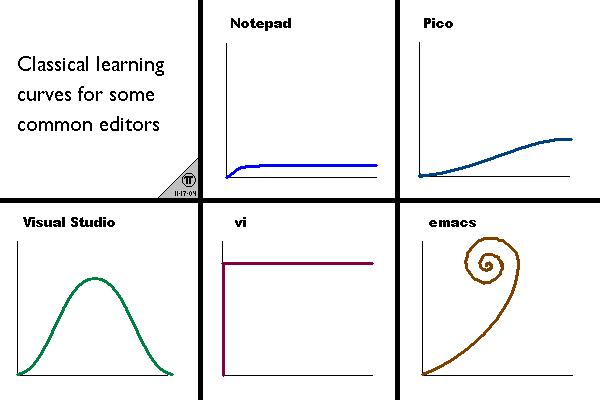
\includegraphics[scale = .7]{curves.jpg}
\end{frame}

\section{Why use vim?}

\begin{frame}
    \frametitle{Why use vim?}
    \begin{itemize}
	\item (Dramatically) increased editing speed
	\item Quick to load, low resource usage
	\item Edit multiple files in tabs/view splits 
	\item Syntax highlighting/plugin/scripting support
	\item Gui mode available
    \end{itemize}
\end{frame}

\begin{frame}
    \frametitle{Increased editing speed}
    \begin{itemize}
	\item All commands are keyboard driven
	\begin{itemize}
	    \item Hands stay on the home row
	    \item No need to use mouse
	    \item Not having to use arrow keys or mouse saves a lot of time
	\end{itemize}
	\item Vim is modal
	\begin{itemize}
	    \item Command mode allows commands like save, edit, etc.
	    \item Visual mode facilitates highlighting text
	    \item Normal mode permits text manipulation
	    \item Insert mode is for, well, inserting text!
	\end{itemize}
    \item These ideas may seem foreign, but in practice they're highly
	effective.
    \end{itemize}
\end{frame}

\begin{frame}
    \frametitle{Quick to load, low resource usage}
    \begin{itemize}
	\item Vim is {\bf fast}
	\item Instantaneous startup times
	\item Non-existent resource overhead
	\item Very low graphical overhead
	\item Terminal based, works just fine over ssh
    \end{itemize}
\end{frame}

\begin{frame}
    \frametitle{Edit multiple files}
    \begin{itemize}
	\item Vim allows you to edit multiple files simultaneously
	\item vim foo.c foo.h bar.c bar.h
	\begin{itemize}
	    \item Need to make changes in several files?
	    \item Edit them all at once in one instance of vim
	\end{itemize}
	\item Horizontal/vertical window splits
	\begin{itemize}
	    \item Edit .h and .cpp files in one window
	    \item Edit one file in multiple places with different splits
	\end{itemize}
	\item Vim also supports tabbing
	\begin{itemize}
	    \item vim -p foo.c foo.h bar.c bar.h
	    \item Edit all of your files at once
	    \item Be able to keep track of where you are without switching windows
	\end{itemize}
    \end{itemize}
\end{frame}

\begin{frame}
    \frametitle{Syntax highlighting}
    \begin{itemize}
	\item Understand the structure of code at a glance
	\item Verify that your keywords are spelled correctly
	\item Reduce the amount of thinking you need to do to understand code
    \end{itemize}
\end{frame}

\begin{frame}
    \frametitle{Plugins}
    \begin{itemize}
	\item Add new features and functionality to vim painlessly
	\item Run make inside of vim
	\item If make fails, your cursor will be sent to the line 
	    with the error
	\item Alternate between .c and .h files with a single command
	\item Add a wiki inside vim to organize your notes and 
	    documentation
    \end{itemize}
\end{frame}

\begin{frame}
    \frametitle{Scripting}
    \begin{itemize}
	\item Syntax highlighting and plugins are just instances of scripting Vim
	\item Vim comes with it's own scripting language, vimscript
	\item Allows you to automate/add features as you see fit
	\item Bindings for perl and python available
	\item This makes Vim a highly adaptable editor
    \end{itemize}
\end{frame}

\begin{frame}
    \frametitle{Gvim}
    \begin{itemize}
	\item For those that don't want to jump headlong into a new editor,
	    there is gvim
	\item Gvim is your regular vim, but with buttons, menus, and the normal
	    editor controls that you would expect
	\item Good way to ease into vim instead of jumping in without a 
	    lifejacket
    \end{itemize}
\end{frame}

\section{Demonstration}

\section{Further resources}

\begin{frame}
    \frametitle{Further resources}
    \begin{itemize}
	\item vimtutor - an interactive guide to vim commands
	\item irc.freenode.net \#vim
	\item reddit.com/r/vim
    \end{itemize}
\end{frame}

\begin{frame}
    This presentation was written in Vim and \LaTeXe{} :)
\end{frame}

\end{document}
